
\section{Manifolds, Curvature, and the Euler Characteristic}
\label{sec:cast}


The Gauss-Bonnet theorem is a bridge. On one shore is topology and
on the opposite shore geometry. This bridge can be traveled in both directions.
That is, if one has geometric information one can deduce topological information and
if one has topological information one can deduce geometric information.
In symbols, the theorem can be stated as follows

\begin{equation} \label{eqn:g-b}
\int_M K dA + \int_{\partial M} k_g ds = 2\pi \chi(M).
\end{equation}
In this section, we define these symbols.

\subsection{Preliminaries}

We begin with some definitions a that may already be familiar to the reader,
\begin{definition}[Topological Space \cite{munkres}]
A \EMPH{topology} is a pair $(X,\tau)$, where $X$ is a set and
 $\tau$ is a collection of subsets $X$
satisfying:
	\begin{itemize}
		\item $\emptyset$ and $X$ are in $\tau.$
		\item the union of \emph{any} subcollection of elements in $\tau$ is  in $\tau.$
		\item the intersection of any \emph{finite} subcollection of elements in the $\tau$ is in $\tau.$
	\end{itemize}
A set $X$ with a specified topology $\tau$ is called a \EMPH{topological space}.
\end{definition}

We will work with a special type of topological spaces called manfiolds.

\begin{definition}[Manifold  \cite{tu2011}]
	A topological space $M$ is \EMPH{locally Euclidean of dimension $n$}
	if every point $p$ in $M$has a neighborhood $U$ such that there is  a
	homeomorphism  $\phi$ from $U$ into and open  subset of $\R^n$.
	We call the pair $(U,\phi: U\to \R^n)$ a \EMPH{chart}, $U$ a \EMPH{coordinate neighborhood}
	and  $\phi$ a \EMPH{coordinate map}. 
A \EMPH{manifold} is a Hausdorff, second countable, locally Euclidean space.
\end{definition}

The symbol $M$ in \eqnref{g-b} is a manifold. For the most part, we will consider two dimensional manifolds are called \emph{surfaces}.
We will consider both continuous and discrete objects.
For computational purposes, we often want a combinatorial structure on our manifolds.
This structure will often come in the form a triangulation, which we now define.


\begin{definition}[Independent Points]
Let $v_0,v_1,\ldots,v_k$ be points in $\R^n$. We call them \EMPH{affinely dependent}
if there are real numbers $\alpha_0,\alpha_1,\ldots,\alpha_k$, not all 0, such that
$\Sigma_{i=0}^k \alpha_iv_i=0$ and $\Sigma_{i=0}^k \alpha_i=0.$
Otherwise,  $v_0,v_1,\ldots,v_k$ are \EMPH{affinely independent}.

\end{definition}

\begin{definition}[Simplices]
A \EMPH{simplex} $\sigma$ is the convex hull of a finite affinely independent
set $A$ in $\R^n$. The points in  $A$ are  called vertices, the dimension
of  $\sigma$ is $|A|-1$.  The convex hull of a subset of vertices of a simplex
$\sigma$ is a \EMPH{face} of $\sigma$.
\end{definition}

\begin{definition}[Simplicial Complex]
A nonempty family $C$ of simplices is a \EMPH{simplicial complex} if the following
are satisfied:
\begin{itemize}
\item  Each face of any simplex is a simplex.
\item The intersection of $\sigma_1 \cap \sigma_2$ is a face of both $\sigma_1$ and 
$\sigma_2$.
\end{itemize}


\end{definition}

For many of our applications we will consider a special type of manifold called
a triangular mesh. Meshes are used extensively in graphics.


\begin{definition}[Homeomorphism]
A  \EMPH{homeomorphism}  of topological spaces $(X_1,\tau_1$ and $(X_2,\tau_2)$
is a bijection $\phi:X_1\to X_2$ such that for every $\phi$ and $\phi^{-1}$ are continuous.
\end{definition}
For two topological spaces $X$ and $Y$ if there exists a  homeomorphism between
$X$ and $Y$ we say $X$ and $Y$ are topologically  equivalent and write  $X\cong Y.$

\begin{definition}[Triangulation]
For a topological space $X$ and simplicial complex $C$ if $X\cong C$,
then $C$  is a \EMPH{triangulation} of $X$.
\end{definition}

In graphics, it is often useful to approximate smooth surfaces with fine triangulations called
a \emph{mesh}. We will see meshes in many of our applications.

\subsection{Curvature}
Continuous:

Discrete:

Recall that the sum of the interior angles of a triangle is $\pi$,
see \figref{angles} for proof. By induction, the sum of the interior angles
of a convex polygon with $n$ edges is  $(n-2)\pi$, see \figref{angles}
for an example.

\begin{figure}[htb]
\centering
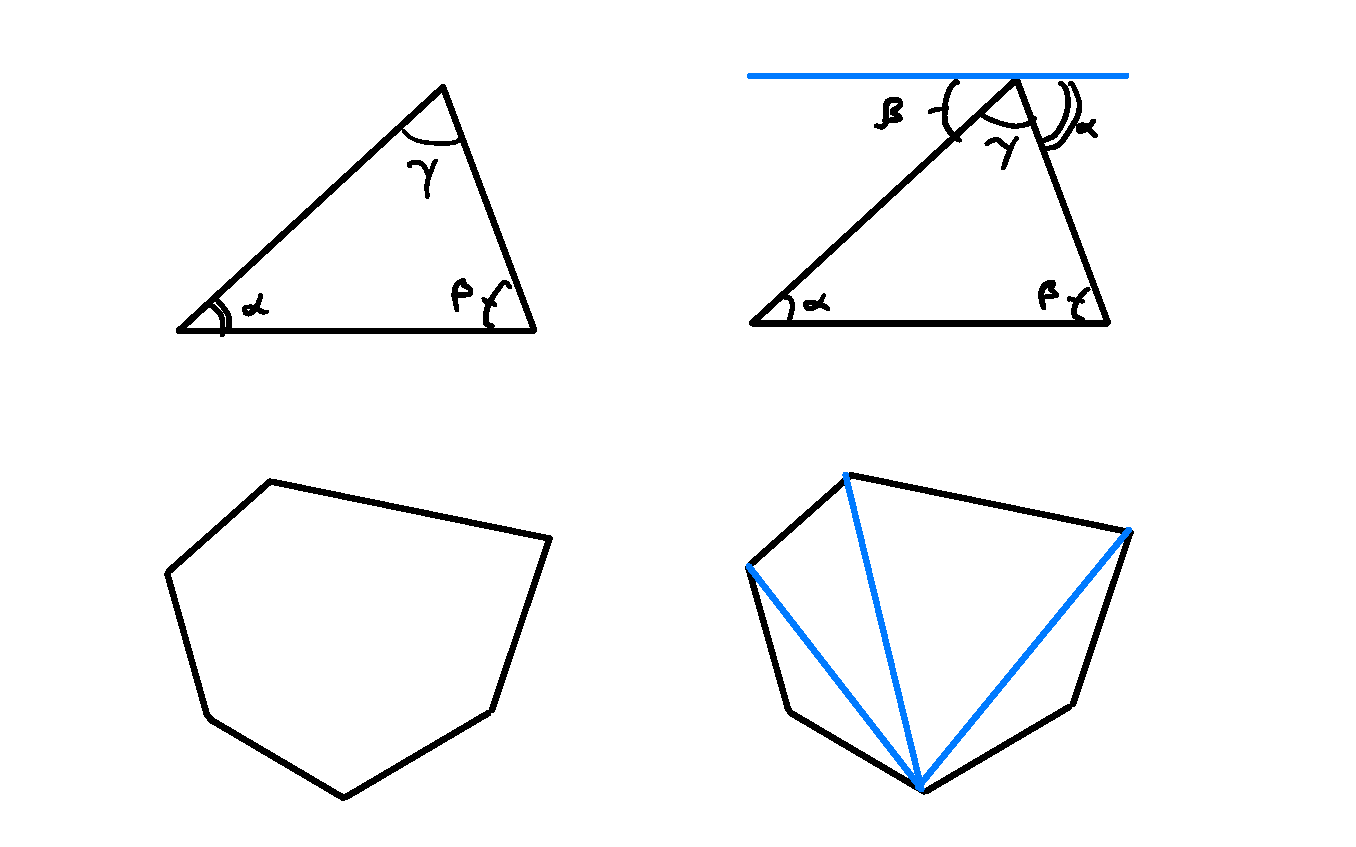
\includegraphics[width=.3\textwidth]{curvature/convex-angles}
\caption{Top row: the sum of  the interior angles of a triangle is $\pi$.
Bottom row: the sum of the interior angles of a convex polygon on $n$ edges is $(n-2)\pi$.}
\label{fig:angles}
\end{figure}


There are several ways to define curvature in the discrete setting \cite{Crane:2013},
this definition will be used in the poof of the discrete Gauss-Bonnet in \secref{proof}.

''For a discrete planar curve we can define the curvature at a vertex as the distance on the unit circle between the two adjacent normals'' \cite{Crane:2013}.

\begin{definition}[Discrete Gaussian curvature \cite{upadhyay2015}]\label{def:discrete-curvature-vertex}

The discrete \EMPH{Gaussian curvature} at a vertex $v$ is the area on the unit sphere bounded by a spherical polygon whose vertices are the unit normals of the faces around $v$.

\end{definition}


\begin{figure}[htb]
\centering
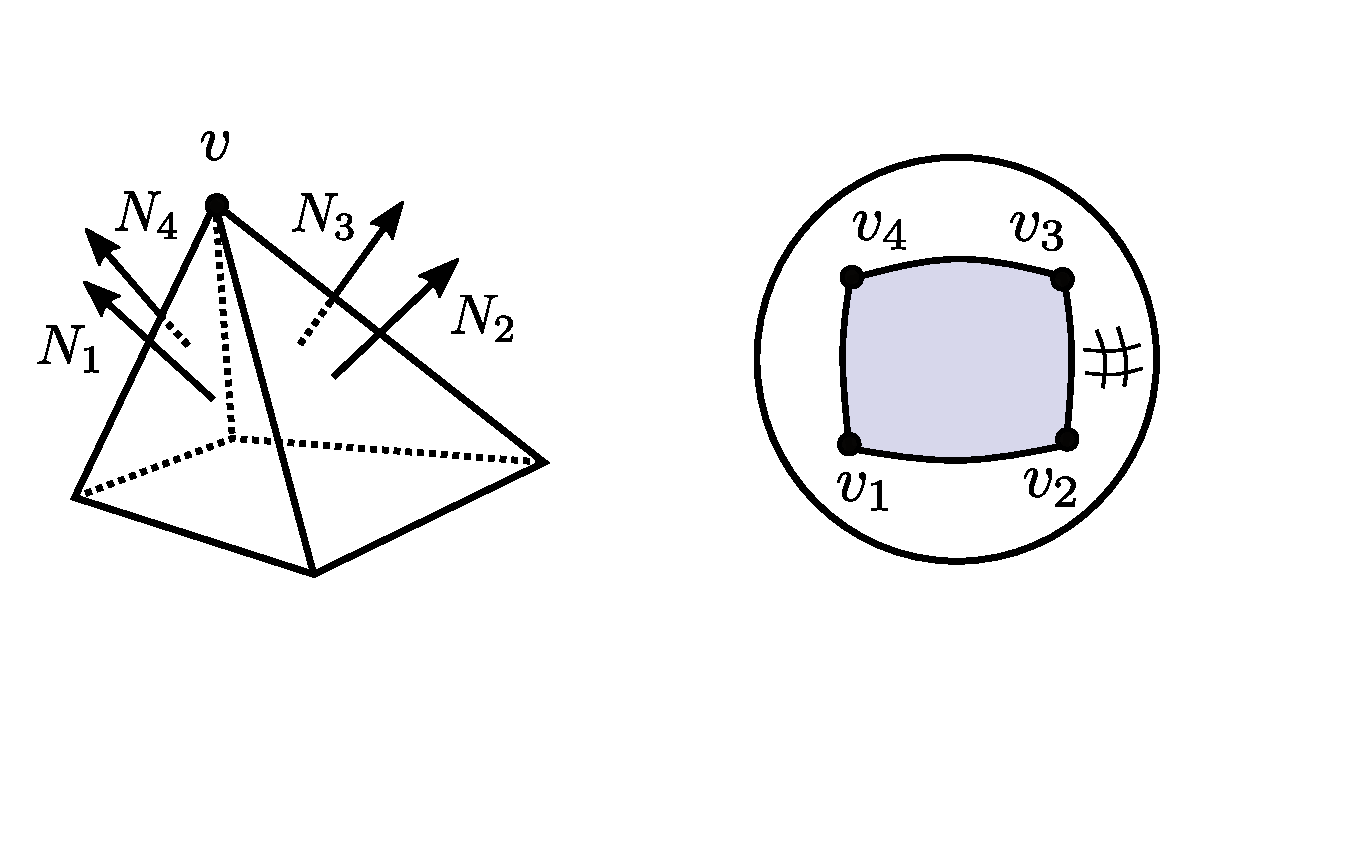
\includegraphics[width=.3\textwidth]{curvature/discrete-curvature}
\caption{The discrete curvature at vertex $v$ is the area drawn on the sphere.}
\label{fig:discrete-curvature}
\end{figure}

The \EMPH{angle defect} at a vertex $d(v)$ is the difference between $2\pi$ and
the sum of the incident angles.  Let $F_v$ denote the faces containing $v$  
and let $\alpha_f$  denote the interior  angle of face $f$ at $v$, then
$$d(v):=2\pi -\sum_{f\in F_v}\alpha_f.$$

The angle defect is equal to the discrete curvature in \defref{discrete-curvature-vertex}.

\subsection{The Euler Characteristic}

Properties of topological spaces that remain unchanged by homeomorphisms are called
\EMPH{topological invariants}. One such invariant is the Euler characteristic.
Originally defined for polyhedra, the \EMPH{Euler Characteristic} for surfaces $\chi$ is the 
the number of vertices minus the number of edges plus  the number of faces, $\chi=V-E+F.$
In higher dimensions, for a triangulated space $X$ the Euler characteristic is 
$\chi(X)=k_0-k_1+k_2-k_3+\ldots$ where $k_n$ is the number of simplices of dimension $n.$
A  graph  is \EMPH{planar} if it can be drawn in the plane with intersections only occuring
at vertices.
For a planar graphs $V-E+F=2$, Eppstein maintains a collection of proofs of this \cite{eppstein-proofs}.
We include the the following proof from Eppstein's list attributed to Thurston
 \cite{thurston}. For any planar graph we can map the graph on to the two sphere
 using stereographic projection.
 
\begin{theorem}[Euler Characteristic for Planar Graphs]\label{thm:euler}
For any planar graph on the 2-sphere we have $V-E+F=2.$
\end{theorem}

\begin{proof}
If needed, perturb the triangulation so that the north and south poles are 
inside of a two faces and there are no vertical edges. At each vertex place a unit positive
charge, at the center of each edge place a unit negative charge and put a unit positive
charge in the middle of each face. Slam the sphere on the ground so that all charges
on the edges and vertices are moved into the face below them. For faces that do not contain a pole
the net charge will be zero, the northern boundary consists of an alternating sequence
of edges and vertices  beginning  and ending with an edge.
The face containing the north pole has a unit positive charge, and the face containing the south
pole contains positive four units of charge and negative three units of charge.
Thus, the total charge is two.

\end{proof}
